\documentclass[11pt]{article}

% Handle Spanish seamlessly!
\usepackage[utf8]{inputenc}
\usepackage[spanish, es-tabla]{babel}

% Change the language for the captions and default names
\renewcommand{\figurename}{Figura}

% Needed for the multline environment
\usepackage{amsmath}

% Images
\usepackage{graphicx}
\graphicspath{{Img/}}

\usepackage{geometry}
\geometry{
    a4paper,
    left = 20mm,
    right = 20mm,
    top = 15mm,
    bottom = 15mm
}

% Links please!
\usepackage{hyperref}

% Format the links
\hypersetup{
    pdfborder = {0 0 0},    % Remove the ugly border
    colorlinks = true,      % Let there be color
    citecolor = black,      % Make citations appear normal (i.e black)
    linkcolor = black,      % The same for links (i.e table of contents)
    urlcolor = cyan         % Color the web links. (cyan is fancy for blueish...)
}


\title{Reparto de tráfico con routers \texttt{CISCO}}
\author{Pablo Collado Soto \\ \\ \textit{Ingeniería de Tráfico}}
\date{}

\begin{document}
    \maketitle

    \section{Introducción}
        En esta práctica estudiaremos los mecanismos de reparto de tráfico de los routers \texttt{CISCO}. En una primera instancia lo haremos con equipos virtuales para luego generar el tráfico con las máquinas virtuales tal y como veníamos haciendo en las prácticas anteriores.

    \section{Pruebas con equipos virtuales}
        Tras realizar la configuración que se explica en el guión de la práctica llegamos a una topología como la que aparece en la figura \ref{fig:topology}. Además de configurar las direcciones \texttt{IP} así como el protocolo de encaminamiento \texttt{OSPF} hemos activado el reparto de tráfico en \texttt{R1}. Dado que todo el tráfico es generado por el \texttt{PC1} solo debemos configurar este reparto de tráfico en \texttt{R1} porque en \texttt{R2} todo lo que llegue saldrá por la interfaz \texttt{e1/0}.\\

        \begin{figure}
            \centering
            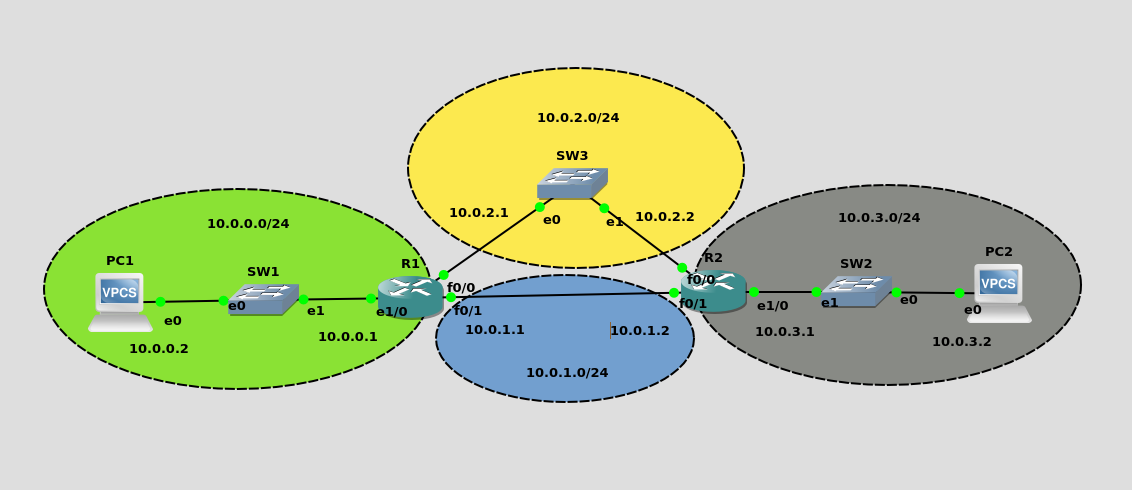
\includegraphics[width=0.6\linewidth]{topology.png}
            \caption{Topología bajo estudio en la primera parte.}
            \label{fig:topology}
        \end{figure}

        \subsection{Reparto de tráfico por destino (PD)}
            Al configurar el reparto de tráfico éste será \textit{por destino} por defecto. Para poder juzgar si este reparto de tráfico está funcionando correctamente empezaremos por mostrar las estadísticas de paquetes emitidos por cada una de las ``cubetas'' del router. Esperamos observar que todas las cubetas estén a $0$ en un inicio como se observa en la figura \ref{fig:ogPktStats.png}. Después mandaremos una serie de \texttt{ping}s desde el \texttt{PC1} al \texttt{PC2} y observaremos que los $5$ paquetes son asociados a una de las ``cubetas'' en función del \texttt{hash} del destino tal y como se comenta en el guión. Si \texttt{ping}eáramos la misma dirección de nuevo observaríamos que los paquetes salen por la misma cubeta al ser el destino idéntico. Podemos observar ésto en la figura \ref{fig:ping1PktStats}. Si después mandamos una serie de \texttt{ping}s a la dirección \texttt{10.0.3.1}, la interfaz del router que pertenece a la subred asociada al \texttt{PC2} estaremos cambiadno el destino, con lo que esperamos que los paquetes salgan por la otra interfaz con mismo coste a la anterior. Los primeros \texttt{ping}s salen por la interfaz \texttt{FastEthernet0/1} asociada a la dirección \texttt{10.0.1.2} como se observa en la figura \ref{fig:ping1PktStats} mientras que los siguientes salen por la interfaz \texttt{FastEthernet0/0} asociada a la dirección \texttt{10.0.2.2} como apreciamos en la figura \ref{fig:ping2PktStats}.\\

            \begin{figure}
                \centering
                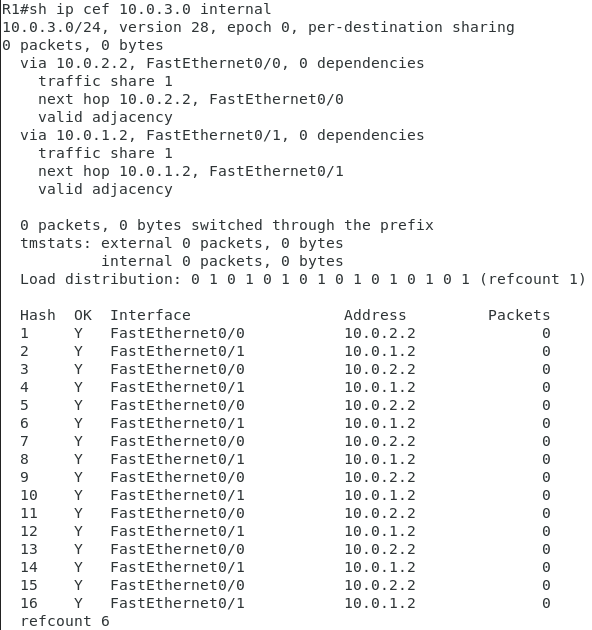
\includegraphics[width=0.6\linewidth]{ogPktStats.png}
                \caption{Estadísticas de paquetes antes de mandar ningún \texttt{ping}.}
                \label{fig:ogPktStats}
            \end{figure}

            \begin{figure}
                \centering
                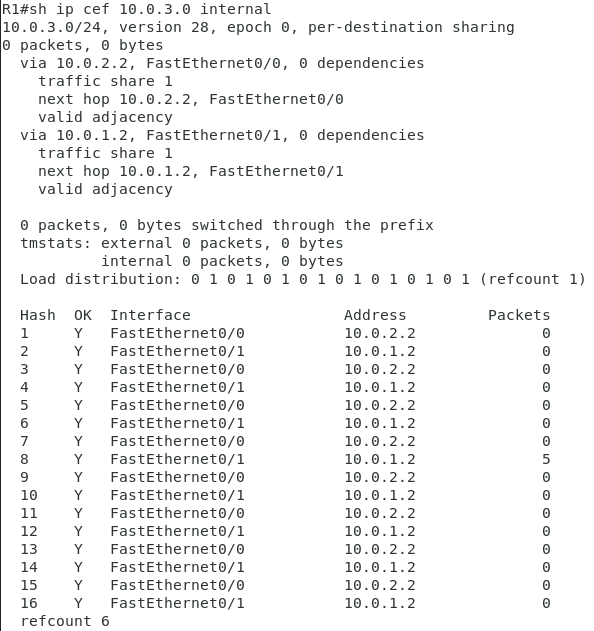
\includegraphics[width=0.6\linewidth]{ping1PktStats.png}
                \caption{Estadísticas de paquetes tras los primeros $5$ \texttt{ping}s.}
                \label{fig:ping1PktStats}
            \end{figure}

            \begin{figure}
                \centering
                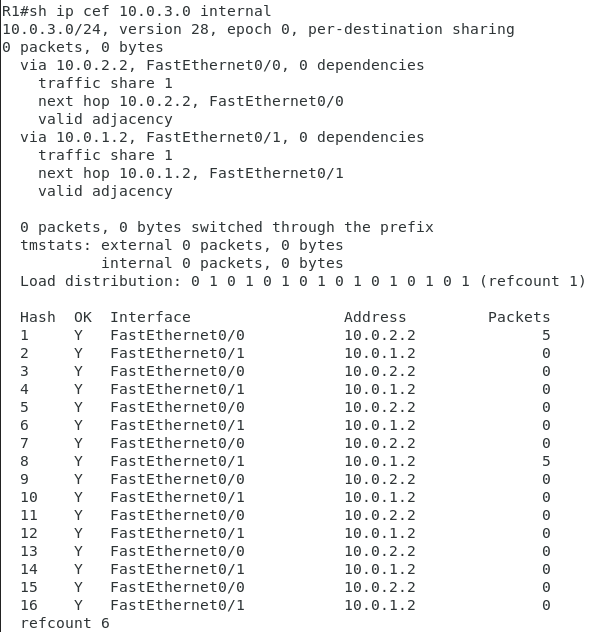
\includegraphics[width=0.6\linewidth]{ping2PktStats.png}
                \caption{Estadísticas de paquetes tras los segundos $5$ \texttt{ping}s.}
                \label{fig:ping2PktStats}
            \end{figure}

            Con esto concluimos que el reparto de tráfico por rutas de igual coste basándonos en el destino de los paquetes funciona correctamente. Como curiosidad señalamos que el primer par de \texttt{ping}s se pierden por un \textit{timeout} debido a que al estar las tablas de \texttt{ARP} vacías se deben popular en toda la red, proceso que introduce una latencia.

        \subsection{Reparto de tráfico por paquetes (PP)}
            Para configurar el reparto de tráfico por paquetes debemos simplemente especificarlo en la terminal de configuración para sobrescribir el comportamiento por destino que se aplica por defecto. El estado de las estadísticas de paquetes tras aplicar este nuevo reparto de tráfico sigue siendo el que encontrábamos en la figura \ref{fig:ping2PktStats}. Tras volver a \texttt{ping}ear al \texttt{PC2} observamos las estadísticas de paquetes de nuevo y llegamos al resultado de la figura \ref{fig:ping3PktStatsPP}. Debemos recordar que, sin opciones adicionales, enviamos $5$ \texttt{ping}s con lo que veremos que aparecen $5$ paquetes adicionales en las estadísticas. Como ahora el reparto tiene una granularidad a nivel de paquete asistimos a unas estadísitcas que envían cada paquete por una de las interfaces de manera alterna. El primero de todos va asociado al \texttt{hash} $1$ y sale por la interfaz \texttt{FastEthernet0/0} y el quinto, asociado al \texttt{hash} $5$, es emitido también por la interfaz \texttt{FastEthernet0/0}. Vemos que la interfaz de salida se alterna con cada paquete. Nótese que el primer contador es $6$ porque partimos del escenario anterior mostrado en la figura \ref{fig:ping2PktStats}. De todo esto concluimos que el reparto por paquetes también funciona.\\

            También hemos realizado las pruebas propuestas ejecutando un \texttt{trace 10.0.3.2} desde \texttt{PC1} y viendo que la dirección \texttt{IP} del segundo salto varía entre \texttt{10.0.1.2} y \texttt{10.0.2.2} tal y como cabría esperar con el balanceo que hemos configurado. Con el balanceo por destino este salto no cambiaría porque el destino de los paquetes emitidos sería siempre el mismo...

            \begin{figure}
                \centering
                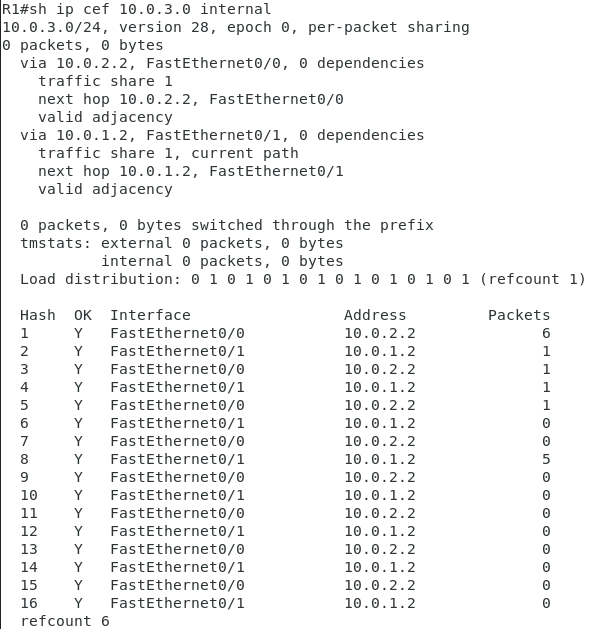
\includegraphics[width=0.6\linewidth]{ping3PktStatsPP.png}
                \caption{Estadísticas de paquetes tras los primeros $10$ \texttt{ping}s.}
                \label{fig:ping3PktStatsPP}
            \end{figure}

        \subsection{Deshabilitando el reparto de tráfico}
            Al deshabilitar el reparto de tráfico perdemos la capacidad de ejecutar el comando \texttt{show ip cef 10.0.3.0 internal} con lo que dependemos de la información mostrada por \texttt{show interfaces stats}. Debemos recordar que en las estadísticas mostradas por este comando tenemos ``ruido'' de fondo introducido por protocolos como \texttt{OSPF} que envían mensajes de manera periódica. Ésto supone que si ejecutamos este comando en dos instantes distintos veremos cómo la los contadores de paquetes emitidos por interfaz crecen a un ritmo lento pero positivo aún sin haber emitido ningún tráfico de usuario desde el \texttt{PC1}. Para poder observar de manera más clara lo que ocurre con el tráfico de usuario modificaremos la invocación de \texttt{ping} para aumentar el número de mensajes y la cadencia con la que estos se emiten para así esclarecer las estadísticas que podemos obtener.\\

            Para conseguir nuestro objetivo ejecutaremos el comando \texttt{ping 10.0.3.2 -c 500 -i 1} con lo que enviaremos $500$ pings a una cadencia de $1\ ms$. El comportamiento que observamos es que todo el tráfico sale por una interfaz determinada. Incluimos la tabla de encaminamiento de \texttt{R1} en la figura \ref{fig:R1Routes} en la que se observa que la primera ruta al destino sale por la interfaz \texttt{FastEthernet0/0} asociada a la dirección \texttt{10.0.2.2} Ésta es la interfaz cuyo contador de paquetes emitidos se dispara tras someterla a una prueba de estrés con el comando \texttt{ping} modificado. De estos resultados deducimos que todo el tráfico se envía por la interfaz asociada a la primera ruta en la tabla de encaminamiento de \texttt{R1}. La elección de la interfaz podría ser aleatoria (desconocemos la implementación del sistema de los routers \texttt{CISCO}) pero creemos que como decíamos se escoge la primera entrada de la tabla de encaminamiento. En cualquier caso, si comparamos el estado inicial de la figura \ref{fig:ifaceStatsNoBalancingStart} con el final de la figura \ref{fig:ifaceStatsNoBalancingEnd} nos daremos cuenta de que el contador de la interfaz \texttt{FastEthernet0/0} ha crecido muchísimo más que el de la interfaz \texttt{FastEthernet0/1} con lo que deducimos que, en ausencia de balanceo de carga todo el tráfico sala por una interfaz (\texttt{FastEthernet0/0} en nuestro caso) aunque haya dos cuyo coste al destino sea el mismo.

            \begin{figure}
                \centering
                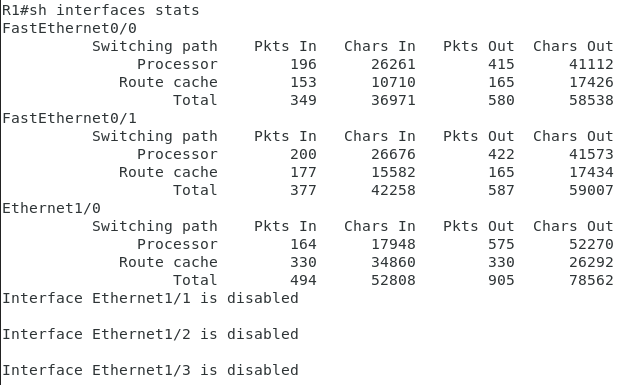
\includegraphics[width=0.6\linewidth]{ifaceStatsNoBalancingStart.png}
                \caption{Estadísticas de paquetes por interfaz antes de emitir tráfico de usuario.}
                \label{fig:ifaceStatsNoBalancingStart}
            \end{figure}

            \begin{figure}
                \centering
                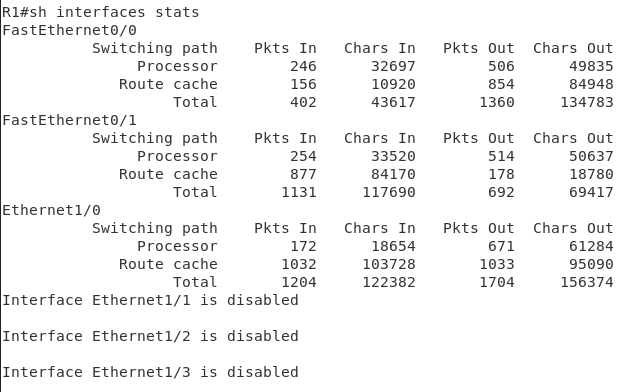
\includegraphics[width=0.6\linewidth]{ifaceStatsNoBalancingEnd.png}
                \caption{Estadísticas de paquetes por interfaz tras emitir tráfico de usuario.}
                \label{fig:ifaceStatsNoBalancingEnd}
            \end{figure}

    \section{Reparto con routers reales}
            Tal y como se indica en el guión de la práctica ahora vamos a generar tráfico con \texttt{mgen} y estudiar las gráficas que obtenemos. ASumiremos que el equipo que genera tráfico es \texttt{SRC} y el que lo recibe será \texttt{DST}.

            \subsection{Prueba sin reparto de tráfico}
                En este caso veremos que todo el tráfico que enviemos desde \texttt{SRC} a \texttt{DST} seguirá la misma ruta a través del ``rombo'' en mitad de la topología. Como los enlaces de dicho rombo están limitados a $10\ Mbps$ veremos cómo esta es la cota superior de la velocidad para ambos protocolos de transporte. En el caso de \texttt{UDP}, tal y como se ve en la figura \ref{fig:udpTraffNoBalancingR}, esta tasa de $10\ Mbps$ se mantendrá durante los $2\ s$ que dura el flujo. Como la tasa del enlace por el que se desaloja el tráfico es menor que la tasa del flujo ($22\ Mbps$) la cola de salida asociada a esta interfaz se irá llenando hasta provocar el descarte de paquetes. Tras finalizar el flujo se vaciará esta cola, cosa que explica la tasa no nula entre los segundos $2$ y $3$ donde el \texttt{SRC} ya no está emitiendo ningún tráfico. Podemos corroborar nuestras sospechas viendo que la latencia se satura rápidamente y que la tasa de pérdidas es prácticamente constante en todo momento ya que muchos de los paquetes emitidos por \texttt{SRC} se encuentran una cola llena.\\

                En el caso de \texttt{TCP}, tal y como vemos en la figura \ref{fig:tcpTraffNoBalancingR}, la tasa se comporta de manera parecida a la de \texttt{UDP}. La principal diferencia radica en que el intervalo de tiempo en el que mantenemos una tasa de $10\ Mbps$ es mayor ya que la propia operativa del protocolo ``alarga'' la ráfaga de tráfico para garantizar que llegue al receptor en su totalidad. Es por ello que observamos una tasa de pérdidas nula tal y como garantiza \texttt{TCP} por diseño.\\

                En definitiva vemos que a grandes rasgos la tasa del flujo se limita a $10\ Mbps$ por los enlaces que conforman el rombo de la topología. Debido a este hecho, \texttt{UDP} perderá tráfico pero su ráfaga acabará ``a tiempo'' mientras que \texttt{TCP} transmite todo el tráfico, pero lo hace en un tiempo no predecible \textit{a priori}.

                \begin{figure}
                    \centering
                    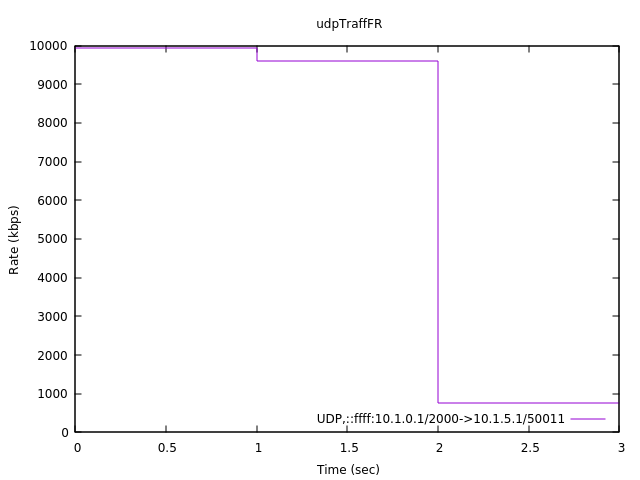
\includegraphics[width=0.6\linewidth]{udpTraffNoBalancingR.png}
                    \caption{Tasa del flujo \texttt{UDP} sin reparto de tráfico.}
                    \label{fig:udpTraffNoBalancingR}
                \end{figure}

                \begin{figure}
                    \centering
                    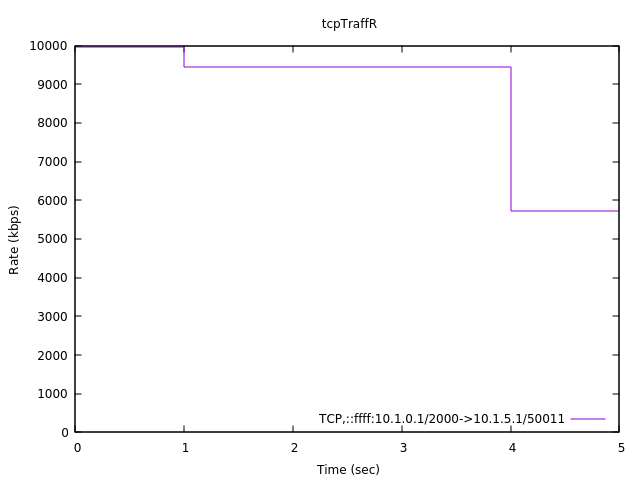
\includegraphics[width=0.6\linewidth]{tcpTraffNoBalancingR.png}
                    \caption{Tasa del flujo \texttt{TCP} sin reparto de tráfico.}
                    \label{fig:tcpTraffNoBalancingR}
                \end{figure}

            \subsection{Prueba con reparto de tráfico por paquete (PP)}
                
\end{document}
